\newpage
\section{Przegląd istniejących rozwiązań w zakresie sztucznej skóry}
\label{s_przeglad}

\subsection{Dostępne metody wykrywania dotyku}

Podstawą w budowie sztucznej skóry jest możliwość wykrywania bodźców zewnętrznych. O ile pomiary temperatury, pod względem dalszej użyteczności, nie muszą posiadać dużej rozdzielczości pomiaru o~tyle rzecz ma się całkiem inaczej jeśli chodzi o wykrywanie nacisku. To właśnie miejsce i siła nacisku jest kluczową informacją jakiej oczekujemy od sztucznej skóry. W zależności od przeznaczenia i możliwości, do budowy wykorzystywane są różne materiały oraz metody produkcji. Do wykrywania nacisku wykorzystywane są różne zjawiska mechaniczne, elektryczne a nawet chemiczne. Istnieją także różnice w~sposobie przesyłania sygnałów w samym czujniku, jak i do układu sterowania robotem. Wszystkie wybrane metody powinny ze sobą współpracować i się uzupełniać wewnątrz wybranego rozwiązania.

Zazwyczaj wyborem, do którego dostosowywane są pozostałe jest sposób wykrywania i pomiaru siły nacisku. To on definiuje możliwości i typy użytej warstwy ochronnej. On~również definiuje jakie układy elektroniczne zostaną użyte do obsługi sztucznej skóry oraz sposób połączenia czujników nacisku z elektroniką sterującą. Możliwych metod pomiaru nacisku jest wiele, ale najbardziej powszechnymi są:
\begin{itemize}
    \item pojemościowe - pomiar zmieniającej się pojemności,
    \item rezystancyjne - pomiar zmieniającej się rezystancji,
    \item piezoelektryczne - pomiar skokowych zmian napięcia,
    \item indukcyjne - pomiar zmian natężenia pola magnetycznego,
    \item optyczne - pomiar natężenia światła lub jego barw składowych.
\end{itemize}

Do tych rzadziej spotykanych należą niewątpliwie układy MEMS o małym rozmiarze oraz dużo większym stopniu skomplikowania. Spotykane też są rozwiązania hybrydowe, które oprócz standardowych metod pomiaru wspomagają się układami MEMS oraz żywymi komórkami i tkankami \cite{b_article_reviev_tactile_skin}. Nie są to jednak rozwiązania, które aktualnie są stosowane w robotyce ze względu na swój koszt oraz skomplikowanie w wytwarzaniu.

Czujniki pojemnościowe są najprawdopodobniej najczęściej wykorzystywane do pomiaru nacisku. Ich główną zasadą działania jest pomiar pojemności pomiędzy dwoma warstwami przewodnika oddzielonymi dielektrykiem. W praktyce zmiana pojemności wywoływana jest przez zmianę grubości dielektryka (uginanie go) \cite{b_konf_kaczka_przekroj}. Zmiana grubości tej okładki wynika bezpośrednio z przyłożonego do sztucznej skóry nacisku. Czujniki pojemnościowe są tak często wybierane ze względu na swoją wysoką czułość, łatwość budowy, dużą rozdzielczość oraz odporność mechaniczną. Czujniki te wymagają jednak do pracy specjalistycznych układów elektronicznych znanych jako CDC (capacitance to digital converter), które niewątpliwie utrudniają zastosowanie w praktyce \cite{b_article_reviev_2_tactile_skin, b_konf_wloch_1_opis_budowy}.

Innym również często spotykanym sposobem wykrywania nacisku jest wykorzystanie zmieniającej się rezystancji materiału pod wpływem nacisku. Rozróżniane są tutaj czujniki piezorezystancyjne oraz tensometryczne, przy czym te drugie, ze względu na zależność od fizycznego odkształcenia czujnika, są rzadko wykorzystywane. Wykorzystywane i~budowane są natomiast czujniki w oparciu o wykorzystanie materiałów piezorestywnych i pomiarze zmian ich rezystancji w zależności od przyłożonej siły. Pozwala to na skonstruowanie czujnika o praktycznie dowolnej wielkości i kształcie. Układ pomiarowy, w~przeciwieństwie do czujników pojemnościowych, jest bardzo prosty, a same pomiary bardzo czułe na zmiany. Niestety układy mierzące rezystancję pobierają z reguły dużo prądu, co czyni je nie najlepszym wyborem w zastosowaniach o niskim zużyciu energii. Układy te również cechują się stosunkowo długim czasem pomiaru i dużą rozbieżnością pomiarów \cite{b_article_reviev_tactile_skin, b_article_reviev_2_tactile_skin, b_konf_tactile_resist_review}.

W robotyce do pomiaru nacisku spotykane jest także wykorzystywanie czujników piezoelektrycznych. Zbudowane są one ze specjalnych polimerów, które pod wpływem nacisku generują ładunek elektryczny lub napięcie, które jest później mierzone. W zależności od zmierzonej wartości można wnioskować jak mocna wystąpiła zmiana nacisku. Czujniki piezoelektryczne nadają się jednak tylko do pomiarów dynamicznych - nie są w~stanie wykryć statycznie przykładanej siły. Ta cecha może być zaletą, ponieważ eliminuje konieczność kalibracji do warunków podczas uruchamiania. Zazwyczaj jednak jest to wada, ponieważ nie jesteśmy w stanie wykryć nawet dużych sił, jeśli nie zmieniają one swojej wartości. Są to natomiast czujniki bardzo odporne na czynniki środowiskowe i~zapewniają bardzo szybki odczyt \cite{b_article_tactile_piezo, b_article_reviev_tactile_skin, b_article_reviev_2_tactile_skin}.

Czujniki indukcyjne również są wykorzystywane do wykrywania nacisku. Ich działanie polega na tworzeniu pola magnetycznego z wykorzystaniem cewek i monitorowaniu jego zmian. Przyłożenie nacisku powoduje ugięcie powierzchni przewodzącej prąd, jednocześnie zmieniając właściwości pola magnetycznego wewnątrz czujnika. Te właśnie zmiany są wykrywane i ich charakterystyka wykorzystywana jest w dalszej obróbce sygnału. Pomiar ten zapewnia szybkie i stosunkowo dokładne pomiary nacisku. Największą wadą czujników indukcyjnych, wykluczającą ją z większości zastosowań, jest konieczność stosowania w środowisku wolnym od materiałów wpływających na pole magnetyczne. Poza tym układy te pobierają sporo energii, a do ich obsługi potrzebna jest specjalistyczna elektronika \cite{b_article_tactile_inductive, b_article_reviev_tactile_skin}.

Ostatnim z najczęściej spotykanych sposobów pomiaru nacisku są czujniki optyczne i te bazujące na pomiarze zmiany parametrów wiązki światła. Ogólna zasada działania jest bardzo prosta i polega na wysyłaniu wiązki świetlnej przez przezroczysty ośrodek, a~następnie odbieranie wiązki z drugiej strony ośrodka. Ośrodek ten jednak jest podatny na nacisk i pod jego wpływem zmienia swoje właściwości, deformując przechodzącą przez niego wiązkę światła. Deformacje te mogą polegać na zmianie ilości przepuszczanego światła lub jego widmie. Czujniki te są w~stanie wykrywać bardzo małe siły oraz są w~pełni odporne na zakłócenia pochodzące ze środowiska zewnętrznego.
Budowa czujnika musi być jednak wykonana bardzo precyzyjnie, aby nie pogarszać właściwości czujnika i~zachować niewielkie rozmiary (czujniki optyczne są trudne i drogie do zminiaturyzowania) \cite{b_konf_tactile_opto, b_article_reviev_tactile_skin, b_article_reviev_2_tactile_skin}.


\subsection{Modułowa sztuczna skóra przeznaczona dla robotów humanoidalnych}

%Co, gdzie, czy i jak działa, wady zalety, zastosowanie

Jednym z lepiej wykonanych i szeroko testowanych przykładów sztucznej skóry jest ten rozwijany we Włoszech na Uniwersytecie Genueńskim. Jest to projekt rozwijamy od wielu lat, który w założeniach miał być stosowany w robotach humanoidalnych jako dodatkowe zabezpieczenie podczas pracy. Jednym z głównych efektorów robota humanoidalnego są manipulatory, które z uwagi na swoją charakterystykę pracy posiadają ruchome stawy, które to znacząco utrudniają wykorzystanie sztucznej skóry w okolicach zgięć robota. Dodatkowo, manipulatory posiadają zazwyczaj dużą potencjalną powierzchnię kolizji, która dodatkowo mocno się zmienia podczas pracy robota \cite{b_konf_wloch_1_opis_budowy}. 

Aby sprostać tak wysokim wymaganiom, do budowy sztucznej skóry zostały wybrane czujniki pojemnościowe wraz z przemysłowymi przetwornikami CDC (capacitance to digital converter, przetwornik pojemnościowo-cyfrowy). Dużą uwagę położono także na modułowości wybranego rozwiązania i możliwości bardzo łatwej i szybkiej rozbudowy całego systemu poprzez wykorzystanie większej liczby modułów. Na zbudowanym prototypie zostało także przeprowadzone szereg badań pod kątem zależności odczytów od~czynników zewnętrznych. Badania te pokazały dobrą stabilność pomiarów i pozwoliły na wykonanie dokładnej charakterystyki sztucznej skóry 
\cite{b_article_wloch_4_wytrzymalosc, b_konf_wloch_1_opis_budowy}. Przekrój budowy pojedynczego modułu czujnika oraz sposób łączenia modułów ze sobą został przedstawiony na rysunku \ref{f_triangle_1-2-3}. Na zdjęciach można zauważyć jak blisko siebie położone są kolejne pola pomiarowe. Warstwa dielektryka pełni w tym rozwiązaniu nie tylko funkcję przenoszenia informacji, ale również chroni robota przed potencjalnymi uszkodzeniami. Takie rozłożenie pozwoliło zrealizować na kolejnych etapach prac miarodajne i rzetelne badania \cite{b_konf_wloch_1_opis_budowy}.

\begin{figure}[!h]
  \begin{subfigure}[t]{0.55\linewidth}
    \centering
    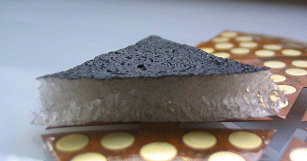
\includegraphics[width=0.95\linewidth]{img/triangle2.png}
    \caption{Budowa pojedynczego modułu sztucznej skóry} 
    % \vspace{4ex}
  \end{subfigure}
  \begin{subfigure}[t]{0.4\linewidth}
    \centering
    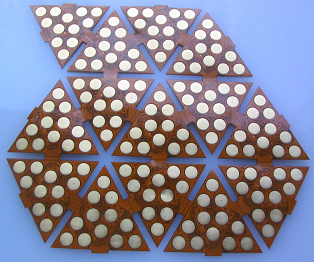
\includegraphics[width=0.83\linewidth]{img/triangle3.png}
    \caption{Sposób łączenia modułów sztucznej skóry} 
    % \vspace{4ex}
  \end{subfigure}
  
  \centering
  \caption{Prototyp modularnej sztucznej skóry projektowanej do robota humanoidalnego \cite{b_konf_wloch_1_opis_budowy}}
  \label{f_triangle_1-2-3}
\end{figure}

Zaprojektowane rozwiązanie zostało w praktyce przetestowane na robocie Baxter, na jednym z jego ramion, gdzie zostało zamocowane aż 768 czujników pojemnościowych \cite{b_site_baxter}. Na umieszczonym tak prototypie zostały wykonane testy idące dużo dalej niż samo wykrywanie nacisku. Na podstawie danych otrzymywanych z modułów rozpoznawane były kształty, jakie są przykładane do robota, czym w przypadku testów było różne ułożenie dłoni na robocie. Surowe dane przed dalszą obróbka są przekształcane do postaci obrazu trójwymiarowego uwzględniającego położenie każdego z czujników w przestrzeni.
Na tym etapie uwzględniane są także położenia poszczególnych stawów robota względem siebie, co pozwala na prawidłową identyfikację nacisku w stawach robota.
Do celów rozpoznawania wzorców na sztucznej skórze została wykorzystana konwolucyjna sieć neuronowa osiągająca skuteczność do $97\%$
\cite{b_konf_wloch_2_reka, b_konf_wloch_3_reka}. Na rysunku \ref{f_triangle_test} jest widoczna sztuczna skóra zamocowana na robocie oraz jej testy na robocie.

\begin{figure}[!h]
  \begin{subfigure}[t]{0.36\linewidth}
    \centering
    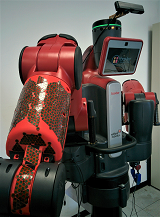
\includegraphics[width=0.95\linewidth]{img/triangle4.png}
    \caption{Robot Baxter z zamocowaną podstawą sztucznej skóry} 
    % \vspace{4ex}
  \end{subfigure}
  \begin{subfigure}[t]{0.62\linewidth}
    \centering
    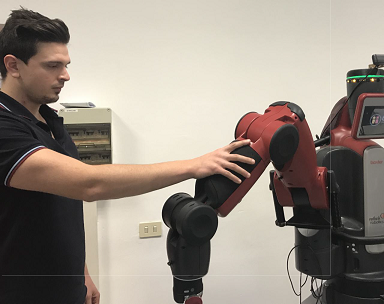
\includegraphics[width=0.95\linewidth]{img/triangle5.png}
    \caption{Sztuczna skóra na robocie podczas testów} 
    % \vspace{4ex}
  \end{subfigure}
  
  \centering
  \caption{Prototyp modularnej sztucznej skóry testowanej na robocie \cite{b_konf_wloch_2_reka}}
  \label{f_triangle_test}
\end{figure}

Zaprojektowane we Włoszech rozwiązanie może w przyszłości być stosowane powszechnie w robotach humanoidalnych. Jest to nie tylko bardzo dobre zabezpieczenie przed wejściem robota w kolizję z otoczeniem lub człowiekiem przy nim pracującym, ale również pozwala na zdalne sterowanie ruchami robota poprzez wykrywanie ułożeń dłoni operatora na skórze robota. Stopień zaawansowania prac nad rozwiązaniem pozwala na założenie, że w ciągu kilku najbliższych lat podobne rozwiązanie pojawi się na rynku. 


% ZA: An Embedded Artificial Skin for Humanoid Robots  Giorgio Cannata, Marco Maggiali, Giorgio Metta and Giulio Sandini

% ZB: On the Recognition of Human Hand Touch from Robotic Skin Pressure Measurements Using Convolutional Neural Networks  Alessandro Albini, Simone Denei and Giorgio Cannata

% ZC: Tactile Images Generation from Contacts Involving Adjacent Robot Links  Alessandro Albini1 and Giorgio Cannata

% ZD: A Flexible and Robust Large Scale Capacitive Tactile System for Robots   Perla Maiolino, Marco Maggiali, Giorgio Cannata, Giorgio Metta, and Lorenzo Natale


\subsection{Elastyczna sztuczna skóra do środowisk współpracy z człowiekiem}

Roboty pracujące pośród ludzi, jak pokazał wcześniej opisany przykład, muszą zapewnić człowiekowi bezpieczeństwo podczas pracy robota. Kluczowe jest więc pokrycie sztuczną skórą wykrywającą nacisk jak największej powierzchni obudowy robota. Pokrycie dużej powierzchni wiąże się jednak z koniecznością użycia dużej liczby czujników i mocy obliczeniowej do przetworzenia w czasie rzeczywistym otrzymywanych danych. Zminimalizowanie tych dwóch czynników jest więc pożądane w przemyśle, aby możliwie mocno zmniejszyć koszty bez straty bezpieczeństwa pracy. Rozwiązanie tego problemu zostało zaproponowane przez naukowców z kanadyjskiego Uniwersytetu Lavala w Quebec. Ich głównymi założeniami przy projektowaniu sztucznej skóry były niski koszt wytworzenia i~możliwość szybkiej reakcji na otrzymane bodźce
\cite{b_konf_gietka_przekroj}.
% W przypadku robotów, których przeznaczeniem będzie wykorzystanie do pracy z ludźmi, bardzo istotną kwestią jest bezpieczeństwo podczas interakcji robot-człowiek. Kluczową funkcją, która mogłaby zwiększyć poziom ochrony człowieka przed ewentualnymi wypadkami, jest zapewnienie wykrywania kontaktu na całym ciele robota (lub na jego najbardziej narażonych na kolizję z człowiekiem elementach). Nad tym problemem pochylili się naukowcy pracujący w Departamencie Inżynierii Mechanicznej Uniwersytetu Lavala w Kanadzie. Dodatkową motywacją stojącą za zaproponowanym przez nich projektem było wyprodukowanie stosunkowo niedrogiej powłoki, która byłaby w stanie zapewnić przestrzenną lokalizację kolizji robota z otoczeniem i szybką reakcję na nią. Rozwiązanie, które skonstruowali, to w praktyce cienki elastyczny arkusz czujnika wykonany z folii poliimidowych z tuszem przewodzącym prąd oraz gumową warstwą wrażliwą na nacisk. Poza niską ceną, dużą zaletą zaproponowanego rozwiązania jest brak konieczności prowadzenia przewodów wewnątrz czujnika. Problem ten ominięty został przez zastosowanie przewodzącego tuszu. Zaproponowany obwód mocno minimalizuje liczbę przewodów wyjściowych \cite{b_konf_gietka_przekroj} \cite{b_book_gietka_source_1}.% CITE AS: a, b

Zastosowany czujnik swoje działanie opiera na pomiarach rezystancji specjalnej folii znajdującej się wewnątrz. W zaproponowanym rozwiązaniu, dwie przewodzące płaszczyzny są oddzielone od siebie materiałem wrażliwym na nacisk. Bez obciążenia zewnętrznego posiada on bardzo dużą rezystancję, która wraz z przykładaniem coraz większego nacisku stopniowo się zmniejsza. Same przewodzące płaszczyzny są w praktyce równolegle ułożonymi pasmami przewodzącymi. Pasma na przeciwnych płaszczyznach są~ułożone względem siebie prostopadle. Cały schemat budowy jest dobrze zobrazowany na rysunku \ref{f_przeglad_gietka_przekroj}, który prezentuje schematyczne ułożenie poszczególnych warstw wewnątrz czujnika. Na zewnątrz widoczne są~także warstwy ochronne czujnika znajdującego się wewnątrz. Dużą zaletą zaproponowanego rozwiązania jest wykorzystanie specjalnych tuszów przewodzących prąd, co pozwoliło na znaczne ograniczenie konieczności stosowania przewodów. Zbudowany czujnik został dodatkowo zalany w żywicy, aby uodpornić go na warunki zewnętrzne i~zapewnić większą trwałość \cite{b_konf_gietka_przekroj}.

\begin{figure}[!h]
    \centering 
    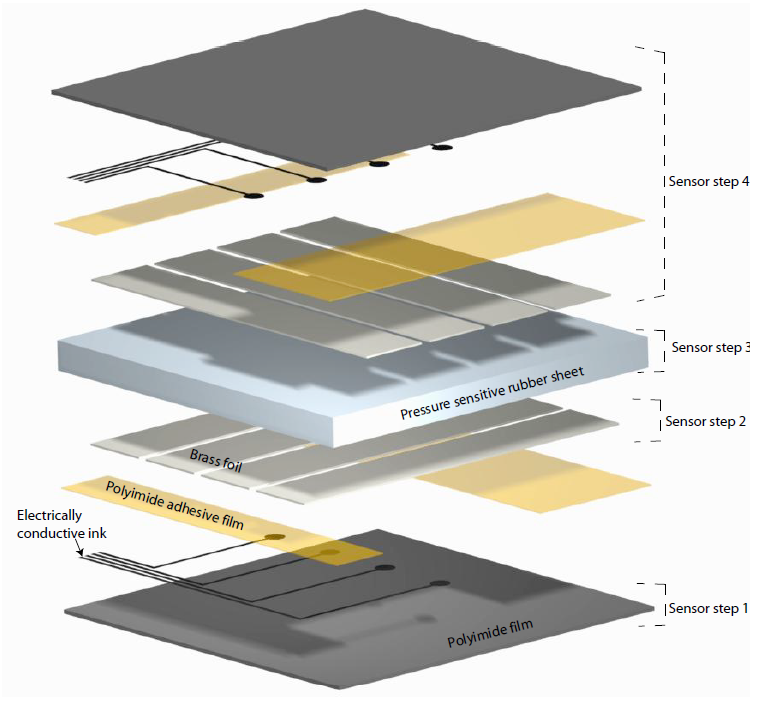
\includegraphics[width=0.4\linewidth]{img/przekroj_gietka.png}
    \caption{Schemat ułożenia poszczególnych warstw sztucznej skóry \cite{b_konf_gietka_przekroj}}
    \label{f_przeglad_gietka_przekroj}
\end{figure}


% Następnie, czujnik został osadzony między dwoma warstwami poliuretanu o różnej twardości Shore'a (30A oraz 20A) przy użyciu technologii osadzania kształtu (ang. \textit{shape deposition manufacturing}, SDM). Badacze wykorzystali takie rozwiązanie, aby zapewnić jak najlepsze tłumienie kolizji oraz wytrzymałość mechaniczną. Wytworzona w ten sposób warstwa skóry może w małym stopniu wyginać się bez tworzenia się uszkodzeń. Zauważono jednak, że powyżej pewnego wygięcia wewnętrzne naprężenia materiału mogą aktywować czujnik, co powoduje otrzymanie błędnych odczytów informujących o kontakcie robota z przeszkodą. Rozwiązaniem tego problemu może być wytwarzanie skóry w zakrzywionej formie. % CITE AS: c 
% tu można dodać rys ze schematem tego zatapiania, ale no nie wiem. Ja bym dodała, ale z pierwszym rysunkiem już tego jest około 1 strony opisu 

Na wykonanym prototypie przeprowadzono szereg testów mających na celu określenie zalet i wad wykonanego rozwiązania, jak również wyznaczenie jego charakterystyki pracy. Ogólne testy przebiegły pomyślnie i nie wykazały większych wad poza faktem, że prototyp przy mocniejszym zginaniu wysyła sygnały mogące świadczyć o kontakcie z przeszkodą, której nie ma. Jest to spowodowane tym, że czujnik nie rozpoznaje pochodzie naprężeń obecnych na swojej powierzchni. Rozwiązaniem tego problemu może być wytwarzanie skóry, która naturalnie posiada swoją krzywiznę \cite{b_konf_gietka_przekroj}.

Opisywane rozwiązanie jest dobrym krokiem w kierunku produkcji taniej powłoki wykrywającej kontakt na robotach przemysłowych, lecz przed doprowadzeniem go do użycia komercyjnego potrzebne jest wykonanie dalszych badań. Ten prototyp był w dużej mierze inspiracją i jedną z podstaw do zbudowania prototypu czujnika opisywanego w~kolejnych rozdziałach pracy.

% Po wykonaniu prototypów przeprowadzono serię eksperymentów, aby zweryfikować wartość progową nacisku na wytworzoną skórę. Siła aktywacji czujnika, którą należało przyłożyć, wahała się od $0,5 N$ do $5 N$ dla powierzchni styku $32 mm^2$, co skutkowało progowym ciśnieniem w granicach $15,8 kPa$ do $158 kPa$. Różne odczyty uzyskiwano w zależności od miejsca przyłożenia siły. Wartość progowa nacisku jest funkcją grubości materiału, użytego rodzaju materiału warstwy zewnętrznej, gęstości z basowej warstwie zewnętrznej (twardości warstwy poliuretanu) oraz właściwości fizycznych warstwy materiału wrażliwego na nacisk umieszczonego między płytkami przewodzącymi. Przez zmianę właściwości tych parametrów w projekcie można więc dostosowywać wartości progowej do pożądanych wielkości. % CITE AS: a

% a: V. Duchaine, N. Lauzier, M. Baril, M.-A. Lacasse and C. Gosselin. "A flexible robot skin for safe physical human robot interaction". Robotics and Automation 2009. ICRA '09. IEEE International Conference on, pp. 3676-3681, May 2009. (mat pokonferencyjne)

% b: M. R. Cutkosky, R. D. Howe, and W. R. Provancher, “Force and tactile sensors,” Springer Handbook of Robotics, pp. 455–476, 2008.

% c: M. Hatanaka and M. Cutkosky, “Process planning for embedding flexible materials in multi-material prototypes,” DETC ASME, Chicago, Illinois, USA, September, 2003. (mat pokonferencyjne)


\subsection{Sztuczna skóra wysokiej rozdzielczości wykorzystywana w chwytakach}

% h jednak nie bedzie cytowane

Roboty wykorzystywane są czasami do przenoszenia lub przekładania różnych przedmiotów. Aby wykonywać to sprawnie potrzebują one odpowiednich chwytaków do chwytania przedmiotów. Dodatkowym plusem są chwytaki wyposażone w sztuczną skórę, która pozwala na rozpoznawanie przedmiotów lub przenoszenie ich z odpowiednią ostrożnością. Sztuczna skóra użyta na chwytakach musi się więc charakteryzować wysoką czułością i elastycznością, aby idealnie dopasować się do podnoszonego przedmiotu.
% Czujniki stosowane w robotach z modułem chwytającym muszą charakteryzować się wysoką wydajnością. W przypadku tego typu rozwiązaniach można napotkać wiele problemów związanych z różną strukturą czy elastycznością łapanych przez roboty obiektów. Wyzwaniem mogą też być takie zdarzenia jak poślizg czy utrata kontaktu. 

Sztuczna skóra dostosowana do tego użycia jest rozwijana na Wyższej Szkole Technologicznej w Montrealu w Kanadzie. Sztuczna skóra została zaprojektowana tak, aby~odpowiednio eliminować kolejne potencjalne problemy w użytkowaniu czujnika. Ogólna budowa czujnika jest bardzo prosta i opiera się na pomiarze pojemności, ale ogromną wagę przyłożono do materiałów i~struktur obudowujących czujnik. Jako dielektryk został wykorzystany standardowy elastyczny materiał (oparty na silikonie), ale uformowany w regularne wypustki, które poprawiają charakterystykę pracy czujnika, zwiększają elastyczność pracy oraz pomagają w utrzymaniu niskiej masy powłoki. 
Przekrój budowy czujnika sztucznej skóry, jak również zasada działania elastycznych wypustek dielektryka przedstawiona jest na rysunku \ref{f_przekroj_duck} \cite{b_konf_kaczka_przekroj}.

% Stworzona przez nich sztuczna skóra swój sukces opiera na zastosowaniu rozwiązania, w którym czujniki statyczne i dynamiczne są zintegrowane w tej samej warstwie czujnika pojemnościowego z umieszczoną bezpośrednio nad nim warstwą mikrostrukturalnego dielektryka. Czujniki statyczne odpowiadają za odczyt informacji o lokalizacji nacisku (zarówno normalnej siły, jak i naprężeń ścinających), podczas gdy czujniki dynamiczne odnoszą się do wszystkich zdarzeń kontaktowych, takicj jak poślizg czy rozpoznawanie obiektów. % CITE AS: g
% ??? 'static and dynamic sensing are integrated in the same layer of capacitive sensor with direct written microstructured dielectric'     czy ja to dobrze tlumacze? 

% Materiał dielektryczny w niniejszym projekcie stanowi warstwa silikonu, w którym umieszczone zostały nanocząsteczki materiału przewodzącego, którym jest tytanian baru ($BaTiO_3$). Wykorzystanie tego połączenia zostało doświadczalnie uzasadnione. W porównaniu z innymi dielektrykami używanymi w podobnych rozwiązaniach tytanian baru wykazał najlepsze właściwości. Nie powodował nadmiernej utraty właściwości fizycznych silikonu, jest ogólnie dostępny i kilkukrotnie tańszy od innych materiałów o podobnych właściwościach.  % CITE AS: i
% Silikon z dodatkiem tytanianu baru wprowadzany jest do formy akrylowej nadającej mu wyjątkowy kształt, który ma kluczowe znaczenie w powodzeniu tego konceptu. Powstała warstwa ma kształt arkusza z równomiernie rozmieszczonymi mikrowypustkami o kształcie ściętego stożka. Każda z wypustek ma podstawę o średnicy $0,6 mm$, płasko ściętą końcówkę o średnicy $0,3 mm$ oraz wysokość $0,5 mm$. Odległość między środkami położonych sąsiadująco wypustek to $1,2 mm$. Strona pokryta wypustkami zwrócona jest w stronę płytki PCB przylegając do niej. Po przyłożeniu ciśnienia wypustki ulegają szybkiej reformacji i rozszerzaniu się dotykając płytki coraz większą powierzchnią. Rysunek \ref{f_przeglad_mikrowypustki} przedstawia schematycznie zachowanie mikrowypustek pod wpływem działania siły na warstwę dielektryka. 

\begin{figure}[!h]
  \begin{subfigure}[t]{0.49\linewidth}
    \centering 
    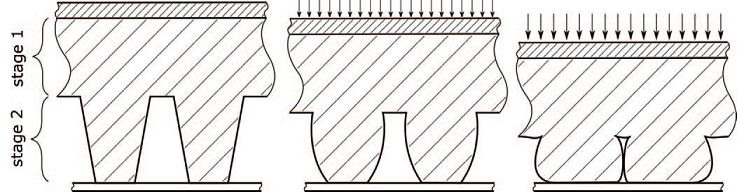
\includegraphics[width=0.95\linewidth]{img/duck_silikon.png}
    \caption{Budowa i działanie wypustek dielektryka}
    % \vspace{4ex}
  \end{subfigure}
  \begin{subfigure}[t]{0.49\linewidth}
    \centering 
    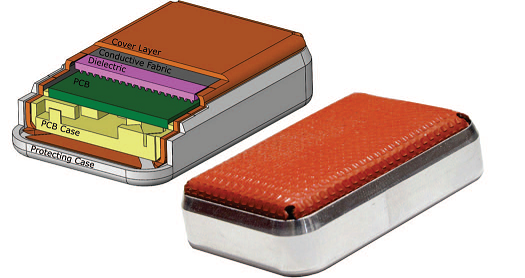
\includegraphics[width=0.95\linewidth]{img/przekroj_duck.png}
    \caption{Przekrój budowy czujnika sztucznej skóry}
    % \vspace{4ex}
  \end{subfigure}
  
  \centering
  \caption{Przekrój budowy dokładnego czujnika sztucznej skóry \cite{b_konf_kaczka_przekroj}}
  \label{f_przekroj_duck}
\end{figure}

Spory uwagę przyłożono także do odpowiedniej budowy części czujnika pojemnościowego znajdującego się na PCB. Zostało przetestowane kilka różnych sposobów prowadzenia ścieżek, które były sprawdzane pod kątem jak najlepszych otrzymywanych odczytów, zarówno statycznych, jak i~dynamicznych. Przeprowadzono również standardowe testy na stabilność pracy w różnych temperaturach, kalibrację czujnika oraz szybkość reakcji. Przeprowadzone doświadczenia potwierdziły zasadność prowadzonych badań oraz doprowadziły do zbudowania pełnego prototypu sztucznej skóry. Prototyp ten został umieszczony do dalszych eksperymentów na chwytaku firmy Robotiq \cite{b_konf_kaczka_przekroj}.

Obserwując postęp prac jest to bardzo obiecujące rozwiązanie, które z powodzeniem będzie wykorzystywane w różnych chwytakach robotycznych ze względu na swoją precyzję oraz elastyczność. Jego głównymi wadami są trudna skalowalność i stosunkowo wysoki koszt produkcji, które to bardzo utrudniają wyposażenie robota w opisywaną sztuczną skórę na całej jego powierzchni.

% wady zalety, zastosowanie

% Zmiany w budowie warstwy przewodzącej nie były jedynymi innowacjami wprowadzonymi przez badaczy do tego projektu. Zaproponowali oni również nowatorski sposób ułożenia sensorów na płytce PCB. Większość dotykowych czujników pojemnościowych posiada kwadratowe taksele. % taxel/pixel - nie wiem jak to przetlumaczyc 
% W przypadku czujników multimodalnych, gdzie należy zastosować dwa typy //takseli??// użycie tego kształtu prowadziłoby do niejednolitej wrażliwości na dotyk w różnych miejscach czujnika. Aby zapobiec temu problemowi zaprojektowano czujnik z //takselami// w kształcie grzebienia, co pozwala na przeplatanie się dwóch rodzajów czujników. % CITE AS: g

% Konstrukcja ta posiada ulepszoną konstrukcję elektryczną i mechaniczną w stosunku do rozwiązań zaproponowanych uprzednio przez innych naukowców. Dzięki temu etap produkcji zostaje uproszczony. Przedstawione rozwiązanie może być z powodzeniem wykorzystane w precyzyjnych robotach wyposażonych w chwytaki. 

\subsection{Sztuczna skóra wykrywająca odkształcenia w trzech osiach}

%Co, gdzie, czy i jak działa, wady zalety, zastosowanie

Ciekawym rozwiązaniem, które może mieć swoje zastosowanie nie tylko w robotyce, ale również w niektórych dziedzinach medycyny, jest projekt w pełni elastycznej sztucznej skóry. Ten wysoce zaawansowany prototyp jest rozwijany na Uniwersytecie Harwardzkim we współpracy z Instytutem Wyssa zajmującego się inżynierią biologiczną. Czujnik ten w~praktyce jest zaawansowanym czujnikiem rezystancyjnym, którego pomiary kolejnych rezystancji są ze sobą mocno skorelowane. 

Zaproponowana sztuczna skóra składa się z trzech warstw mikrokanałów utworzonych w silikonowej formie, które wypełnione są płynną (w temperaturze pokojowej) cieczą przewodzącą prąd. Jako materiał przewodzący wykorzystany został eutektyczny stop galu i indu (EGaIn) \cite{b_article_EGaIn}. Pole czujnika jest małych rozmiarów ($25x25x3,5mm$) oraz jest mocno rozciągliwe. Wymienione cechy pozwalają mu na wykrywanie przykładanego nacisku w~wielu osiach \cite{b_article_tactile_precise}.

Budowa czujnika jest prosta w założeniach, a jej skomplikowanie wynika głównie z~niewielkich rozmiarów pola. Jest on złożony z~kilku warstw silikonowych odlewów z~miejscami na kanały przewodzące, które zostały ze sobą złączone. Każda kolejna warstwa posiada inny kształt kanalików przewodzących, aby wykrywała inne napięcia. Kolejnymi warstwami są: linie horyzontalne, linie wertykalne oraz spirala. Wszystkie kanały są połączone ze sobą w jeden długi kanał z kilkoma wyprowadzeniami na pomiar rezystancji. Po połączeniu ze sobą wszystkich silikonowych warstw mikrokanały wypełniane są, za~pomocą strzykawek, płynnym przewodnikiem.
Zbudowany prototyp czujnika został przedstawiony na rysunku \ref{f_przeglad_prezyzyjna}. Został tam też zaprezentowany schemat warstwowy budowy czujnika \cite{b_article_tactile_precise}.

\begin{figure}[!h]
  \begin{subfigure}[t]{0.495\linewidth}
    \centering
    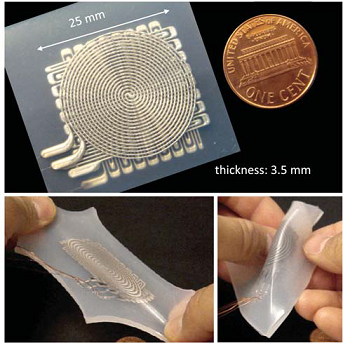
\includegraphics[width=0.9\linewidth]{img/precyzyjna_prezentacja.png} 
    \caption{Prezentacja wykonanego prototypu sztucznej skóry} 
  \end{subfigure}%%
  \begin{subfigure}[t]{0.495\linewidth}
    \centering
    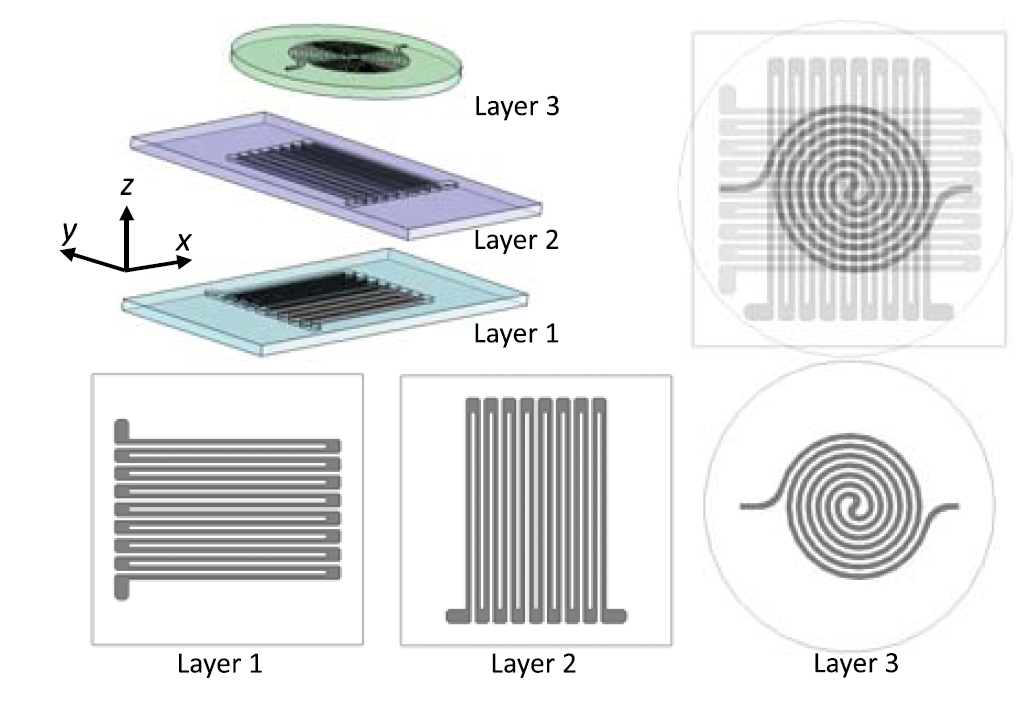
\includegraphics[width=0.95\linewidth]{img/przekroj_precyzyjna.png}
    \caption{Schemat budowy i ułożenia kolejnych warstw czujnika} 
  \end{subfigure}
  \centering
  \caption{Prezentacja i schemat budowy sztucznej skóry z wbudowanymi mikrokanałami \cite{b_article_tactile_precise}}
  \label{f_przeglad_prezyzyjna}
\end{figure}

Podstawowa zasada działania czujnika polega na pomiarze rezystancji poszczególnych kanałów. Mierzona rezystancja wzrasta jeśli kanaliki wypełnione przewodnikiem są rozciągane. Jest to związane ze zmniejszającym się przekrojem kanałów oraz jednocześnie rosnącą ich długością. 
Rezystancja mierzona jest przez pomiar spadku napięcia na poszczególnych warstwach. Zmierzony sygnał jest kolejno wzmacniany i wysyłany na przetworniki analogowo-cyfrowe. Stamtąd jest wysyłany do mikrokontrolera, który może przesłać dane dalej do systemu \cite{b_article_tactile_precise}.
% Doświadczalnie stwierdzono, że czujnik może być rozciągany o $250\%$ bez problemów w pomiarach. Jego rezystancja waha się wtedy od $\sim 2,5 \Omega$ przy braku nacisku do kilkunastu ($\sim12 \Omega$) przy rozciągnięciu o $100\%$. Pomiary są bardzo powtarzalne, ale zawierają histerezę oraz są zależne od szybkości zwiększania przykładanego nacisku 

Opisywany czujnik jest dopiero na początkowym etapie badań i nie posiadał jeszcze dokładnie sprecyzowanego zastosowania. Ze względu na jego budowę i możliwość dopasowania kształtu można go stosować w miejscach o nietypowym kształcie lub małym rozmiarze i przekroju. Sam czujnik może zostać także bardziej zminiaturyzowany lub posiadać inne ułożenie kanalików, które dadzą mu inne możliwości pomiaru napięć.
